\documentclass[11pt,a4paper,notitlepage]{article}

\usepackage[margin=3cm]{geometry}

\usepackage{bookmark}

\usepackage{hyperref}
\hypersetup{colorlinks=true,urlcolor=blue,linkcolor=black}

\usepackage{enumitem}
\setlist[enumerate]{leftmargin=*}
\setlist[itemize]{leftmargin=*}

\usepackage{listings}
\lstset{
  basicstyle=\ttfamily,
  columns=flexible,
  escapechar=@,
  tabsize=4,
  commentstyle=\color{darkgray},
  frame=l,
  framerule=1pt}
\NewDocumentCommand{\mono}{m}{\lstinline{#1}}
\lstnewenvironment{code} {\lstset{language=C}} {}

\usepackage{calc}

\usepackage{float}

\usepackage{booktabs}

\usepackage{xcolor}

\setlength{\parindent}{0pt}
\setlength{\parskip}{.5em}
\setlength{\skip\footins}{2em}

\renewcommand*\familydefault{\sfdefault}

\usepackage{graphicx}
\graphicspath{{img/}}

\usepackage{tcolorbox}
\tcbset{parbox=false}
\newenvironment{infobox} {\begin{tcolorbox}[title=Info]} {\end{tcolorbox}}

\newcommand{\zephyrversion}[0]{3.5.0}
\newcommand{\sdkversion}[0]{0.16.3}
\newcommand{\imagename}[0]{zephyr\_stm32\_v\zephyrversion{}}
\newcommand{\cmdinwsl}[0]{wsl -d \imagename{}}

\newcommand{\maintitle}[0]{Zephyr Development Environment Container}

\NewDocumentCommand{\puttitle}{m}{%
  \begin{center}
    \huge
    \begin{minipage}[b]{.4\textwidth}
      
\includegraphics[height=2.5em]{en-zhaw-ines}
    \end{minipage}%
    \begin{minipage}[b]{.6\textwidth}
      \begin{flushright}
        \textbf{\maintitle}\\
        #1
      \end{flushright}
    \end{minipage}%
    \vspace{1cm}
  \end{center}
  \lfoot{\maintitle{} #1}
}

\usepackage{fancyhdr}
\pagestyle{fancy}
\lhead{}
\chead{}
\rhead{}
\lfoot{}
\lfoot{}
\cfoot{}
\rfoot{\thepage}
\renewcommand{\headrulewidth}{0pt}
\renewcommand{\footrulewidth}{0pt}


\begin{document}

\puttitle{}

\section{Introduction}

These instructions explain the setup of a containerized environment for developing Zephyr applications.
This environment can either be used with a container runtime or the \emph{Windows Subsystem for Linux}.

The \emph{Containerfile} can be found in Appendix~\ref{containerfile} for anyone interested.

The containerized environment only works on x86 architectures.
If your machine has a different architecture, you can get a native Zephyr installation by following the Zepyhr \href{https://docs.zephyrproject.org/\zephyrversion/develop/getting_started/index.html}{Getting Started Guide}.
Beware, that you must ensure to checkout the right Zephyr version. Replace the \mono{west init \~/zehpyrproject} command from the Getting Started Guide by the following command.

\begin{lstlisting}
west init --mr v@\zephyrversion{}@ zephyr_@\zephyrversion{}@
\end{lstlisting}

\section{Technical Background (optional read)}

\subsection{Necessity for WSL or Containers}

In the following labs, you are going to work with the Zephyr RTOS.
By providing a containerized environment, we can ensure a reproducible setup.
Additionally, the images are lightweight, have a small memory footprint, and outperform a conventional VM.

\subsection{Windows Subsystem for Linux}

The Windows Subsystem for Linux (WSL 2) is available for Windows 10/11 since 2019.
Not all Windows Versions include it per default, an installation is possible via the Microsoft Store or \emph{winget}.
WSL 2 runs inside a managed virtual machine (VM) that includes a Linux kernel.
The virtualization is implemented via a highly optimized subset of Hyper-V features.
WSL 2 on Windows 11 can retain up to 95 \% of the performance of a native Linux Distribution.

\subsubsection*{Benefits compared to a conventional VM}

\begin{itemize}
  \item Seamless integration in Windows.
        Files contained within the WSL can be accessed directly via the regular Windows file explorer.
  \item After creating a WSL image, it can be started directly in the file explorer.
  \item The VM setup is seamless and executed automatically without user
        interaction.
\end{itemize}

\subsection{Container Runtime}
Container runtimes are an alternative to the VM that WSL 2 provides.
These runtimes are typically developed for linux systems\footnote{Docker and Podman are available for Windows but run in WSL 2 in the background}.
Two notable container runtimes are \emph{Docker} and \emph{Podman}.

\newpage

\section{Setup with WSL}

Follow these steps to set up a Zephyr development environment in the WSL.

\begin{itemize}
  \item Install the \emph{J-Link Software and Documentation pack}.
        Make sure to tick the \emph{Install legacy USB Driver for J-Link (requires admin rights)} checkbox during installation.

        \href{https://www.segger.com/downloads/jlink/JLink_Windows_x86_64.exe}{Download}

  \item Install \emph{PuTTY} or another application that can be used for serial
        communication.
        Either download from \href{https://putty.org/}{here} or install with \emph{winget}:

        \begin{lstlisting}
winget install --id PuTTY.PuTTY -e
\end{lstlisting}

  \item Optional: install \href{https://aka.ms/terminal}{\emph{Windows Terminal}} for a better terminal experience.

        \begin{lstlisting}
winget install --id Microsoft.WindowsTerminal -e
\end{lstlisting}

  \item Open a terminal.

  \item Ensure that the WSL is installed.
        \begin{lstlisting}
wsl --install --no-distribution
\end{lstlisting}

        \begin{infobox}
          After installing WSL, make sure to reboot your machine.
          Otherwise the changes will not be applied.
        \end{infobox}

        \begin{infobox}
          If you see the help output of \mono{wsl} try without the \mono{--no-distribution} switch.
          If you get an error try installing the WSL from the Windows Store.
          This can either be done with the \emph{Microsoft Store} GUI or with \mono{winget}:

          \begin{lstlisting}
winget install "Windows Subsystem for Linux"
\end{lstlisting}

        \end{infobox}

  \item Create a folder for the environment and import the provided WSL image.
        \begin{lstlisting}
mkdir \path\to\wslDistroStorage\@\imagename{}@
wsl --import @\imagename{}@ `
  \path\to\wslDistroStorage\@\imagename{}@ `
  "$env:USERPROFILE\Downloads\@\imagename{}@_wsl.tar.zst"
\end{lstlisting}

  \item Open a shell inside the environment.

        \begin{lstlisting}
@\cmdinwsl{}@
\end{lstlisting}

        \begin{infobox}
          In case you get a \emph{CreateProcessParseCommon:789: Failed to translate D:\textbackslash} error the file system might not be available from within WSL.
          Run the following command to list the available file systems.

          % \cmdinwsl{ls /mnt}
          \begin{lstlisting}
@\cmdinwsl{}@ ls /mnt
\end{lstlisting}

          You can try mounting the missing file system (\mono{D:\\} in this case) with the following commands.

          \begin{lstlisting}
@\cmdinwsl{}@ mkdir /mnt/d
@\cmdinwsl{}@ mount -t drvfs D: /mnt/d
\end{lstlisting}
        \end{infobox}
        \begin{infobox}
          If you are using \emph{Windows Terminal} you can conveniently open a new tab with the environment.
          You might have to restart the terminal for this option to appear.
          \begin{center}
            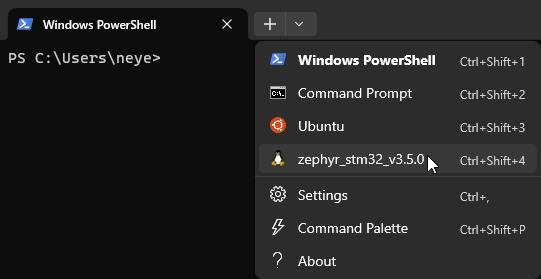
\includegraphics[width=.5\paperwidth]{terminal_open_wsl_tab}
          \end{center}
        \end{infobox}
\end{itemize}

\newpage

\section{Setup with a Container Runtime}

\begin{itemize}
  \item Install the \emph{J-Link Software and Documentation pack (\href{https://www.segger.com/downloads/jlink}{Download})}.
  \item Install a serial terminal like \mono{minicom}.
  \item Install a container runtime (e.g. \emph{podman} or \emph{docker}).
  \item Load the image.
        \begin{lstlisting}
podman load --input @\imagename{}@.tar.zst
\end{lstlisting}
  \item Run the container.
        \begin{lstlisting}
podman run --rm -it \
  -v /path/to/project:/root/dev \
  @\imagename{}@
\end{lstlisting}
\end{itemize}

\newpage

\section{Using the Zephyr Environment}

\subsection{Build Sample}

Run the following inside the environment to compile the blinky sample.

\begin{itemize}
  \item For \textbf{WSL}:
  \begin{lstlisting}
cd ~/zephyrproject/zephyr/samples/basic/blinky/
west build --pristine --board @\board{}@ --build-dir /tmp/build
\end{lstlisting}
  \item For \textbf{Podman/Docker}:
  \begin{lstlisting}
cd ~/zephyrproject/zephyr/samples/basic/blinky/
west build --pristine --board @\board{}@ --build-dir ~/dev/build
\end{lstlisting}
\end{itemize}

\begin{infobox}
  When using WSL, we recommend to include the \mono{--build-dir /tmp/build} argument.
  If omitted the build system will compile the application in a \mono{build} folder in the current directory, which will be very slow when this directory is on the Windows file system (e.g. in \mono{/mnt/c/}).
\end{infobox}

\begin{infobox}
  When using Podman/Docker, setting the build directory to \mono{\~/dev/build} is necessary, otherwise you cannot access the binary from outside the container.
\end{infobox}

% container runtime: make sure builddir accessible

\newpage

\subsection{Flash Sample}

There are two main ways to flash an application to the target.
When first setting up the environment and testing with the blinky sample, you must always use the way described in \autoref{sec:jflash}.
The other way is only applicable if the project provides a \mono{.jlink} file.

\subsubsection{J-Flash Lite}\label{sec:jflash}
Start \emph{J-Flash Lite}, select the target device (\texttt{\mcu}), and make sure the \emph{Internal flash} flash bank is selected.

\begin{center}
  \begin{tikzpicture}
    \node [anchor=south west] {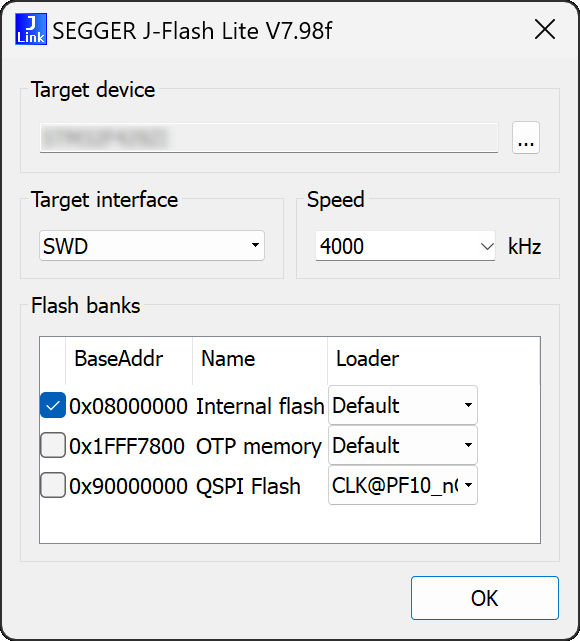
\includegraphics[width=8cm]{jflashlite.png}};
    \draw (7.39,7.1) [red,ultra thick] circle[radius=.4];
    \draw (.84,3.4) [red,ultra thick] circle[radius=.4];
  \end{tikzpicture}
\end{center}

In the next window select the firmware file (\mono{build/zephyr/zephyr.hex}) and click on \emph{Program Device}.

\begin{infobox}
  The WSL file system can be accessed in the explorer.
  \begin{center}
    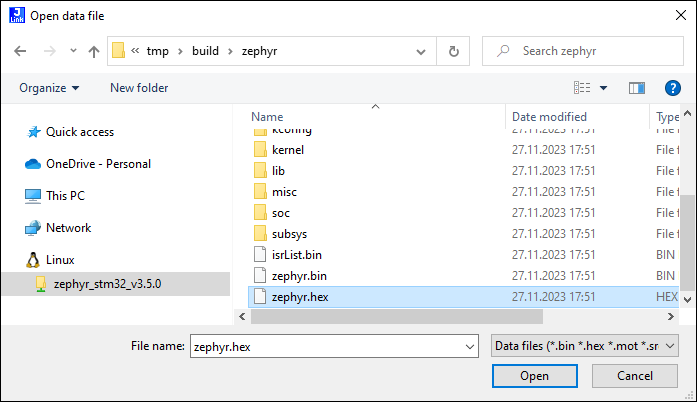
\includegraphics[width=.5\paperwidth]{explorer_wsl_hex}
  \end{center}

  It is possible, that the \emph{Linux} file system does not show up.
  If this is the case, it can be accessed by manually entering its path in the explorer:
  \mono{\\\\wsl\$}
  \begin{center}
    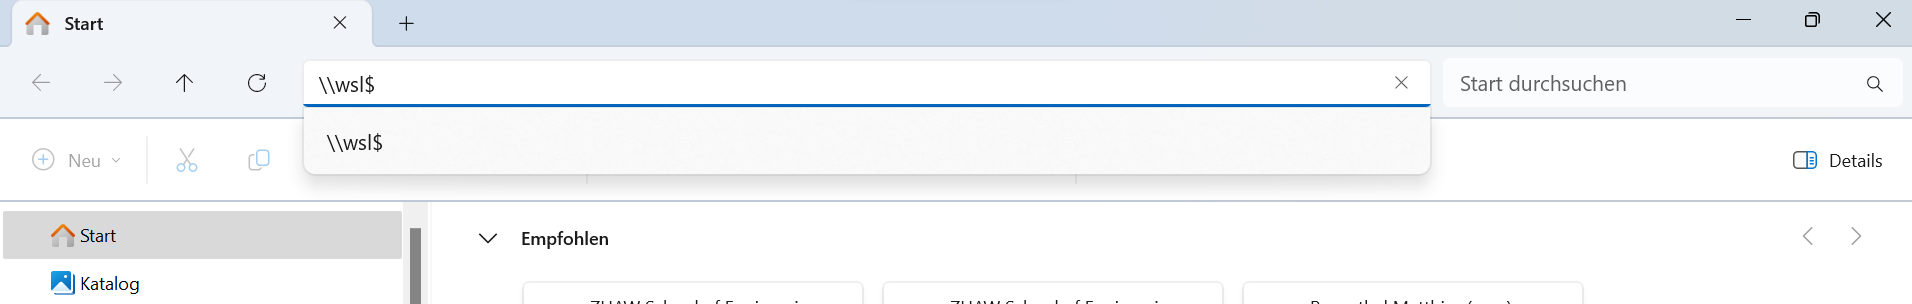
\includegraphics[width=.65\paperwidth]{win_file_explorer_wsl.png}
  \end{center}
  Press \emph{enter} to access the WSL file system.
\end{infobox}

\newpage

\subsubsection{J-Link Command File}
If a J-Link command file (\mono{.jlink}) is present in the project, it can be used to flash the binary from the command line.
On UNIX based systems the command to flash a binary with a J-Link command file is:

\begin{lstlisting}
JLinkExe -CommandFile path/to/file.jlink
\end{lstlisting}

On Windows the path to the J-Link executable needs to be added to the path environment variable first:

\begin{lstlisting}
$env:Path += ";C:\Program Files\SEGGER\JLink_<version>"
JLink -CommandFile path\to\file.jlink
\end{lstlisting}

\begin{infobox}
  Use the file explorer to get the right path to the JLink executable.
\end{infobox}

\begin{infobox}
  The above command to add the path is only for the current session.
  You can also add it permanently if you want.
\end{infobox}

\subsection{Test Flashed Sample}

Open a serial terminal with e.g. PuTTY to see the log output:

\begin{lstlisting}
plink -sercfg 115200 -serial com3
\end{lstlisting}

You might have to press the reset button on your microcontroller board to start the program and print the message again.

\begin{infobox}
  Open the device manager to find the COM-port number.
  \begin{center}
    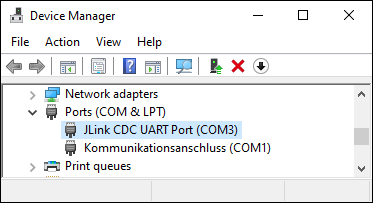
\includegraphics[width=.5\paperwidth]{device_manager_com}
  \end{center}
\end{infobox}

\newpage

\appendix

\fancyfoot{}

\section{Troubleshooting}

\begin{itemize}
\item {\bf Running the Container fails after importing}

  You might need to use \mono{localhost} in the run command:

  \begin{lstlisting}
podman run --rm -it \
-v /path/to/project:/root/dev \
localhost/@\imagename{}@
\end{lstlisting}
\item {\bf The WSL distro is not found after importing}

  Try rebooting your system.
\item {\bf The debug probe keeps announcing itself as mass storage device}

  Open the J-Link shell an disable the mass storage feature.

  \begin{lstlisting}
JLink
msddisable
\end{lstlisting}
\end{itemize}

\newpage
\newgeometry{margin=1cm}

\section{Containerfile}\label{containerfile}

\lstinputlisting[basicstyle=\ttfamily\scriptsize]{../Containerfile}

Usage example:

\begin{lstlisting}
podman build \
  --build-arg="ZEPHYR_VERSION=@\zephyrversion{}@" \
  --build-arg="SDK_VERSION=@\sdkversion{}@" \
  . -t @\imagename{}@
\end{lstlisting}

\end{document}

% Local Variables:
% TeX-output-dir: "build"
% TeX-master: t
% TeX-engine: xetex
% End:
